%%%%%%%%%%%%%%%%%%%%%%%%%%%%%%%%%%%%%%%%%%%%%%%%%%%%%%%%%%
%
% Doctoral Thesis Template @ The University of Manchester
% LaTeX Chapter Template
% Version 1 (23/07/2020)
% Joe Crone
%
% This template is based on:
% The University of Manchester, Presentation of Thesis Policy
% Research Office Graduate Education Team
% June 2017
% http://www.regulations.manchester.ac.uk/pgr-presentation-theses/
%
%%%%%%%%%%%%%%%%%%%%%%%%%%%%%%%%%%%%%%%%%%%%%%%%%%%%%%%%%%
\documentclass[../main.tex]{subfiles}
\begin{document}

% Title
%--------------------------------------------------------
\chapter{CBETA Inverse Compton Scattering Source Design}
\label{CBETA_Inverse_Compton_Scattering_Source_Design} % to reference use \ref{ChapterTemplate}

\section{Motivation for a CBETA Inverse Compton Scattering Source}

\textcolor{blue}{**SHITE BUT GETTING POINTS DOWN**}

The CBETA ERL is the first demonstration of an SRF multi-pass ERL \cite{bartnik2020cbeta}, which enables a compact accelerator to provide 100's~\si{\mega\electronvolt} electron beams with small emittance ($\epsilon_{n} < 1$~\si{\milli\meter}-\si{\milli\radian}) and small relative energy spread whilst maximising beam power. These factors contribute to a high-quality, high-brillance electron beam which is an ideal driver of an inverse Compton source. Consequently, an x-ray light source can be designed to harness CBETA and provide high-quality x-ray beams within a compact footprint. Another advantage of using a multi-pass ERL is that ICS sources can be constructed to use each of the four nominal energies of the CBETA accelerator, therefore a multi-colour radiation source is possible. 

 The maximum electron beam energy of the CBETA at 150~\si{\mega\electronvolt} enables production of x-rays with a minimum wavelength of $\lambda = 0.03$~\si{\angstrom} ($E_{\gamma} = 402$~\si{\kilo\electronvolt}), extending the reach of current synchrotron facilities which are limited to the $E_{\gamma} = 300$~\si{\kilo\electronvolt} range. Smaller wavelength opens up new avenues of application such as tomography of thick specimens and non-resonant inelastic scattering (NIXS) of transition metal oxides -- of relevance to development of high temperature superconductors.
 
 Inherent in the inverse Compton scattering process is a correspondence between photon energy and scattering angle ($E_{\gamma} \propto \theta$), therefore simple collimation is adequate to select a bandwidth of photons from a source. This is even possible once geometric bunch--pulse effects are accounted for. However, this is in contrast to synchrotron and bremmsstrahlung sources, where complicated optical arrangements, like monochromators, are required to select a user specified photon bandwidth. 
 
 Production of narrow-bandwidth radiation is plausible using an ERL ICS source, evidenced by inspection of Eq.~\ref{eq:RMS_bandwidth}, as ERLs such as CBETA have small energy spread and are capable of very small emittances ($\epsilon_{n} = 0.3$~\si{\milli\meter}-\si{\milli\radian}),. Therefore, operation and design of a CBETA inverse Compton scattering source would be informative toward narrow-band radiation sources in the $\gamma$-ray regime, where only bremsstrahlung is competitive as a high-flux source yet suffers from a broad bandwidth and where monochromation is less feasible.
 
 ERLs combine the best of both types of accelerators; they can typically deliver higher-quality beams than those in storage rings, with greater energy efficiency than a linac \cite{smith2006optic}. Therefore, as the beam parameters necessary for scientific research call for higher current and higher quality beams, ERLs are the accelerators best-suited to meet this demand. Multi-turn ERLs, which accelerate the electron beam multiple times before decelerating the beam, have the benefit of being able to reach higher energies without additional cost, power requirements, or floor space \cite{merminga2003high}. Inverse Compton scattering sources benefit from both the high current and high quality electron beams delivered by ERLs which translates into high flux, narrow bandwidth ICS sources. 

\section{ERL Electron Beam and Optical Cavity Laser Pulse Parameters}

Electron bunch parameters for the CBETA inverse Compton scattering source were targeted toward a high brightness electron beam with a low energy spread reflecting our goal of a high average brightness x-ray source with narrow-bandwidth capabilities. For a large flux, a smaller electron beam spot size at the IP is needed; while a larger spot can be beneficial for a narrower scattered photon bandwidth, this ultimately depends on the electron beam divergence. The electron parameters for the design of the CBETA inverse Compton scattering source are majoritively based on the design parameters of the CBETA ERL as presented in the design report \cite{hoffstaetter2017cbeta}. However, these are modified with respect to the considerations relevant to an inverse Compton scattering source and the implications of the multi-pass commissioning \cite{bartnik2020cbeta}. The electron bunch parameters have also been subjected to a series of optimisations, as detailed in Chapter~\ref{Optimisation_and_Characterisation_of_Inverse_Compton Scattering_Spectra}, for premier performance of the CBETA ICS. The optimisations are described later in this section. A baseline case is also presented where the $\beta$-function at the interaction point remains constant across all nominal energies, with a small electron bunch spot size designed to maximise uncollimated flux and brilliance. The electron bunch parameters of the CBETA ICS source are presented in Table~\ref{tab:CBETA_electron_beam_design_parameters}.  

\begin{table}[!h]
\caption{Electron beam parameters envisaged at the CBETA ICS source interaction point (IP). Both baseline and optimised parameters assume a round transverse profile for the electron bunch. The given baseline parameters -- which assume the same $\beta^*$ at the IP -- allow a comparison of flux and bandwidth at different energies. The optimised values beneath those are where we have maximised the flux into a 0.5\% \textit{rms} scattered photon bandwidth through a suitable combination of beam spot size and collimation angle for the round beam optimisation case. }
\vspace{3mm}
\begin{tabular}{lccccc}
\hline\hline
Parameter & \multicolumn{4}{c}{Quantity} & Unit \\
\hline
Turn number & 1 & 2 & 3 & 4 & \\
Electron kinetic energy, $E_e$ & 42 & 78 & 114 & 150 & \si{\mega\electronvolt}\\
Injection kinetic energy, $E_{\mathrm{inj}}$ & \multicolumn{4}{c}{6} & \si{\mega\electronvolt} \\
Repetition rate, $f$ & \multicolumn{4}{c}{162.5} & \si{\mega\hertz}\\
Bunch charge, $e N_e$ & \multicolumn{4}{c}{32} & \si{\pico\coulomb} \\
Transverse normalised \textit{rms} emittance, $\epsilon_{N}$ & \multicolumn{4}{c}{0.3} & \si{\milli\meter}-\si{\milli\radian}\\
\textit{rms} bunch length, $\Delta \tau$ & \multicolumn{4}{c}{1.0 (3.33)} & \si{\milli\meter} (\si{\pico\second})\\
Relative energy spread, $\Delta E_{e}/E_{e}$ & \multicolumn{4}{c}{$5.0\times 10^{-4}$} & \\
\hline
 & \multicolumn{4}{c}{Baseline parameters} & \\
\hline
$\beta^*$ (at the IP) & \multicolumn{4}{c}{1} & \si{\centi\meter}\\
Electron bunch spot size, $\sigma_{\mathrm{electron}}$ & 6.01 & 4.42 & 3.65 & 3.19  & \si{\micro\meter} \\
\hline
 & \multicolumn{4}{c}{Optimised for 0.5\% \textit{rms} bandwidth} & \\
\hline
$\beta^*$ (at the IP) & 3.56 & 6.58 & 9.60 & 12.62 & \si{\centi\meter}\\
Electron bunch spot size, $\sigma_{\mathrm{electron}}$ & 11.34 & 11.34 & 11.34 & 11.34  & \si{\micro\meter}\\
Collimation angle, $\theta_{\mathrm{col}}$ & 1.533 & 0.830 & 0.569 & 0.433 & \si{\milli\radian}\\
\hline\hline
\end{tabular}
\label{tab:CBETA_electron_beam_design_parameters}
\end{table}

The design of the CBETA ERL \cite{hoffstaetter2017cbeta} allows for a maximum bunch charge of 123~\si{\pico\coulomb} whilst the bunch charge assumed in this design is 32~\si{\pico\coulomb}, a factor $\sim$~4 lower. Reduction in bunch charge is necessitated because the coherent synchrotron radiation disruption of the beam imposes a limit on the bunch charge of 32~\si{\pico\coulomb} \cite{lou2020coherent}. The specification of a 162.5~\si{\mega\hertz} repetition frequency, subject to the optical cavity limitations, also means that the average beam current is instantly halved from the design values irrespective of the bunch charge limitations. The maximum average beam current of the CBETA ERL design is 40~\si{\milli\ampere}, this is reduced to 5.2~\si{\milli\ampere} average beam current for operation of the CBETA ICS source. The 5.2~\si{\milli\ampere} average beam current is well within the theoretical current limitations of the beam break-up instability (BBU), simulated to be beyond 40~\si{\milli\ampere} in 98\% of simulations and beyond 1~\si{\milli\ampere} in every simulation performed for the CBETA ERL \cite{lou2019beam}.   

\textcolor{blue}{**BEAM HALO?**}
\textcolor{blue}{**BUNCH LENGTH + LONGITUDINAL DYNAMICS**}

The single-turn commissioning of CBETA \cite{gulliford2021measurement}, successfully demonstrated the operation of the FFA return beamline with electron beams in an energy range from 39 to 59~\si{\mega\electronvolt} \cite{gulliford2019beam,gulliford2021measurement}. Therefore, it is reasonable that the CBETA ERL could be operated within this range to generate ICS photons from the first turn configuration. This would allow production of scattered photons with continuously tuneable energy in the range 27.8 to 63.0~\si{\kilo\electronvolt}. Extending this to the 4-turn configuration, Fig.~\ref{fig:CBETA_ICS_energy_tuning} indicates the possible scattered photon energies using either the nominal energies of the 4 passes, or from the tuneable electron kinetic energy using a single pass. Since tuning of the scattered photon energy of inverse Compton scattering sources is most practical by the variation of the electron beam kinetic energy, Fig~\ref{fig:CBETA_ICS_energy_tuning} is indicative of the likely tuning range at the CBETA ICS or analagously at other multi-pass ERL facilities.  

\begin{figure}[!h]
\centering
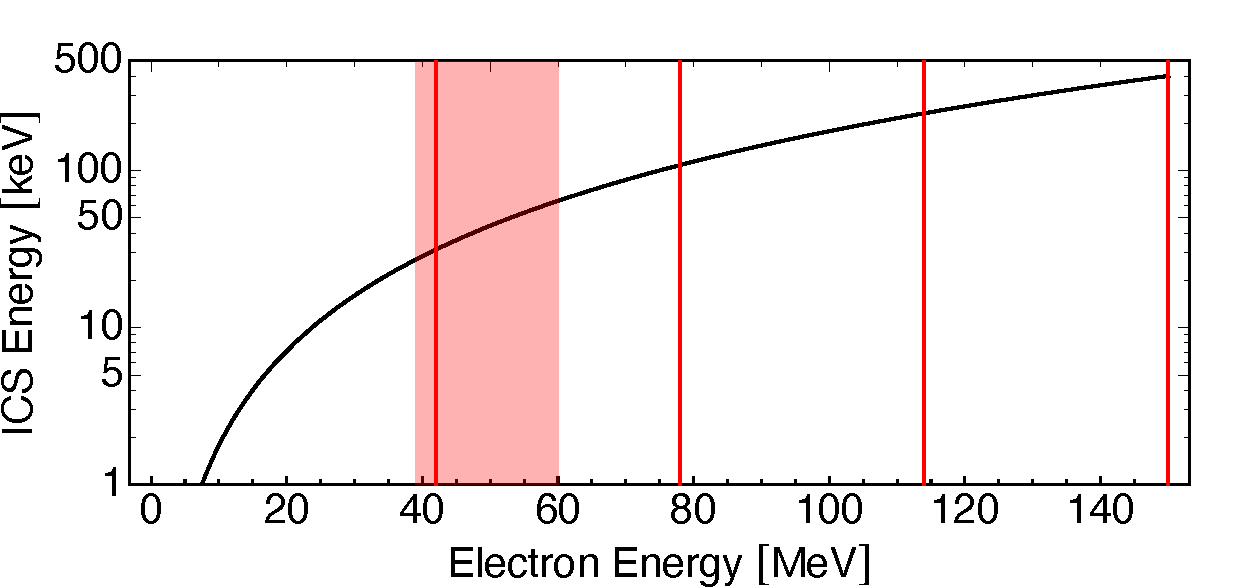
\includegraphics[width=0.7\textwidth]{Figures/CBETA_Inverse_Compton_Source_Design/CBETA_ICS_energy_tuning.pdf}
\caption{An ICS source generating photons from each of the four CBETA ERL passes delivers the (fixed) scattered energies indicated here; we assume a fixed incident laser wavelength of 1064~\si{\nano\meter}. CBETA has also experimentally demonstrated tuning of single-pass acceleration from 39 to 59~\si{\mega\electronvolt} (indicated by the shaded region), which indicates the continuous tuning of scattered photon energy that an ERL in general might deliver. \textcolor{blue}{**RE-DO PLOT?**}}
\label{fig:CBETA_ICS_energy_tuning}
\end{figure}

\textcolor{blue}{**NEEDS EXPANDING AND CHANGING IF I WANT TO USE THE 2D NRB OPT HERE TOO**}
The round beam optimisation result for the $\beta^{*}$ and $\theta_{\mathrm{col}}$ trade-off of a 0.5\% \textit{rms} narrow bandwidth case are shown in Table~\ref{tab:CBETA_electron_beam_design_parameters}. These optimised parameters are the optimum electron bunch interaction point $\beta$-function and collimation angle for maximising the collimated flux of the CBETA ICS into the 0.5\% \textit{rms} bandwidth. The methodology in Section~\ref{sec:RB_optimisation} can be applied to a series of \textit{rms} bandwidth in the range 0--1\% to produce a round beam Pareto front within the $\beta^{*}-\theta_{\mathrm{col}}$ parameter space of the CBETA ICS, as shown in Fig.~\ref{fig:CBETA_beta_theta_parameter_space}.
\begin{figure}[!h]
\centering
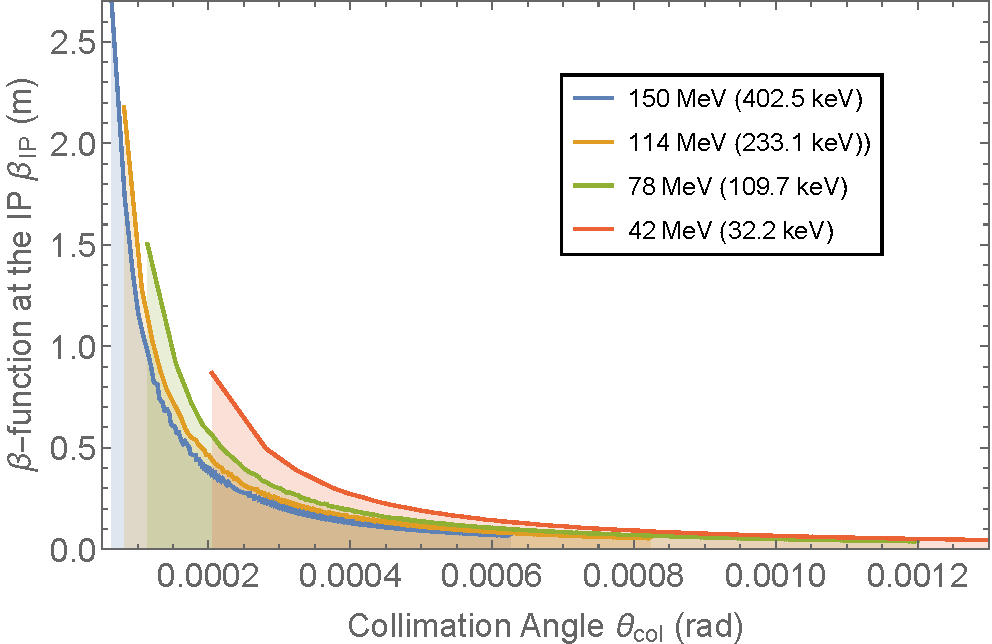
\includegraphics[width=0.7\textwidth]{Figures/CBETA_Inverse_Compton_Source_Design/CBETABetaTheta.pdf}
\caption{Tuning curves of $\beta^{*}$ against $\theta_{\mathrm{col}}$ for each of the nominal CBETA electron beam energies satisfying the maximal flux across the 0--1\% \textit{rms} bandwidth range. The shaded area is the parameter space, while the line corresponds to the maximal flux solution for a given \textit{rms} bandwidth. Minimised bandwidth solutions in this range have large $\beta$-functions at the IP and small collimation angles $\theta_{\mathrm{col}}$; the maximal bandwidth solutions have small $\beta$-functions and larger collimation angles $\theta_{\mathrm{col}}$.}
\label{fig:CBETA_beta_theta_parameter_space}
\end{figure}

Each of the Pareto fronts (for each nominal energy) of the $\beta^{*}-\theta_{\mathrm{col}}$ parameter spaces in Fig.~\ref{fig:CBETA_beta_theta_parameter_space} has a distinctive shape - a linear regime followed by non-linear regime. The Pareto front shows a linear relationship as the collimation angle increases, this part is dominated by the emittance term, until a vertex is reached and, as collimation angle increases, there is a non-linear shape, where the Pareto front is dominated by the collimation term. The termination of the Pareto fronts at the small collimation angle marks the point in which the optimal $\beta$-function at the IP becomes imaginary.

The laser pulse and Fabry-Perot optical cavity parameters are specified in Table~\ref{tab:CBETA_laser_pulse_design_parameters}. For the CBETA ICS a Nd:YAG ($\lambda=1064$~\si{\nano\meter}) laser is specified, which is enhanced and re-circulated by a Fabry-Perot optical cavity. The laser pulse parameters within the optical cavity are based on the Fabry-Perot optical cavity demonstrated in the cERL inverse Compton scattering source \cite{akagi2016narrow}. An identical bow-tie 4-mirror planar cavity is envisioned for the CBETA ICS, a full design of a Fabry-Perot optical cavity was forseen as beyond the scope of this source design. 

A Nd:YAG laser ($\lambda = 1064$~\si{\nano\meter}) is specified for the CBETA ICS as this laser typically has a narrow spectral bandwidth in comparison to other possibilities such as Ti:Sa lasers and Nd:YAG lasers are widely available. A case can be made for a longer wavelength laser, such as a CO$_{2}$ laser \cite{pogorelsky2020converting}, as these incident photons are of lower energy and therefore for a certain pulse energy there is a higher photon density in the interacted pulse which increases the flux of the ICS source. However, the desire for higher energy x-rays makes a Nd:YAG laser with a 1064~\si{\nano\meter} wavelength preferable for this design. In addition, for a high repetition rate of inverse Compton scattering interactions it is necessary to have re-circulation of the laser pulse which requires high-finesse optical mirrors which have been developed more thoroughly in the infrared regime. 

The Fabry-Perot optical cavity repetition rate of the CBETA ICS is set at 162.5~\si{\mega\hertz} because this is the highest repetition rate that has been demonstrated within the ERL environment \cite{akagi2016narrow}. A repetition rate of 325~\si{\mega\hertz} would be ideal as this would allow operation at the nominal CBETA ERL bunch repetition rate \cite{hoffstaetter2017cbeta}. However, in this domain total path length of the cavity (for a single pulse configuration) must be 0.92~\si{\meter} for a 325~\si{\mega\hertz} cavity in comparison to 1.84~\si{\meter} at 162.5~\si{\mega\hertz} which presents engineering challenges such as misalignment of the cavity mirrors and an inevitably larger crossing angle for a planar cavity. Therefore, the more conservative choice of a 162.5~\si{\mega\hertz} interaction repetition rate was selected. The repetition rate of the electron bunches must also match this ratio, hence why the is limited to half of the design bunch repetition rate. 

An Nd:YAG laser typically operates with picosecond \textit{rms} pulse duration, here specified as 10~\si{\pico\second} which is ideal for the CBETA ICS source as this is well matched to the 3.33~\si{\pico\second} electron bunch duration. Picosecond scale pulse duration is advantageous because it diminishes the effect of the hourglass and angular crossing effects \cite{miyahara2008luminosity} whilst also avoiding the timing complexity for the ICS interaction that would be associated with shorter durations. In keeping the average laser power invariant, shorter laser pulse durations would also increase the peak power of the laser upon the Fabry-Perot cavity mirrors which increases the possibility of surface hot-spot defects which reduce average stored power in the optical cavity \cite{wang2020prior}. In addition to this reasoning, the 10~\si{\pico\second} laser pulse duration reflects the pulse duration used in the state-of-the-art 670~\si{\kilo\watt} average stored power optical cavity demonstration with a 1040~\si{\nano\meter} wavelength laser \cite{carstens2014megawatt}.     

An \textit{rms} spot size at the IP of 25~\si{\micro\meter} is proposed as this has been experimentally demonstrated on the cERL ICS experiment \cite{akagi2016narrow}. The cavity used in the cERL experiment also involved a 5\si{\degree} crossing angle, with crossing angles on the degree scale common in many ICS source designs \cite{}. \textcolor{blue}{**need references: ThomX, BriXS etc.**} The proposed spectral bandwidth (relative energy spread of the laser pulse) is not directly stated within the cERL paper \cite{akagi2016narrow}, however based on the pulse duration of the laser, the characteristic small spectral bandwidth of Nd:YAG lasers and the energy selecting nature of a Fabry-Perot cavity an approximation of a 0.7~\si{\nano\meter} \cite{} \textcolor{blue}{**Laura Corner Private Communication} wavelength spread is assumed resulting in a 6.57$\times 10^{-4}$ \textit{rms} spectral bandwidth.     

The Fabry--Perot cavity included within this source design has an average stored power of 10~\si{\kilo\watt}, which is below the state-of-the-art 670~\si{\kilo\watt} stored power demonstration by Carstens et al \cite{carstens2014megawatt}, though this was conducted outside of an accelerator environment. A stable 383~\si{\kilo\watt} average stored power demonstration outside of an accelerator environment has also recently been conducted for the ThomX ICS source \cite{liu2018optical}. In terms of operable optical cavities for ICS, the recent demonstration of the Munich Compact Light Source (MuCLS) operated with a 70~\si{\kilo\watt} average stored power \cite{eggl2016munich}, therefore our parameters are conservative.   
\begin{table}[!h]
\centering
\caption{Nd:YAG Gaussian laser pulse parameters at the CBETA ICS IP. The interacted laser pulse is produced via a Nd:YAG infrared laser and re-circulated in a bow-tie Fabry-Perot optical cavity.}
\begin{tabular}{lcc}
\hline\hline
Parameter & Quantity & Unit \\
\hline
Wavelength, $\lambda_\textrm{laser}$ & 1064 & \si{\nano\meter}\\
Photon energy, $E_\textrm{laser}$ & 1.17 & \si{\electronvolt}\\
Pulse energy  & 62 & \si{\micro\joule}\\
Number of photons, N_{\textrm{laser}} & $3.3\times 10^{14}$\\ 
Repetition rate, $f$ & 162.5 & \si{\mega\hertz}\\
Spot size at the IP, $\sigma_\textrm{laser}$ & 25 & \si{\micro\meter}\\
Crossing angle, $\phi$ & 5 & deg \\
Pulse length  & 10 & \si{\pico\second}\\
Spectral bandwidth, $\Delta E_\textrm{laser}/E_\textrm{laser}$ & 6.57$\times 10^{-4}$ &   \\
 % 0.7nm error on 1064nm
\hline\hline
\end{tabular}
\label{tab:CBETA_laser_pulse_design_parameters}
\end{table}

\section{Bypass Design}
\label{sec:bypass_design}

To utilize CBETA as an inverse Compton scattering source at the 150~\si{\mega\electronvolt} maximum electron beam energy, a bypass line is required that replaces the ordinary 4th pass due to the stringent space restrictions in the existing FFA system; this leaves no space to arrange IP focusing, nor for the laser re-circulation cavity. The scattered photons from the ICS must also be produced in a different plane to the existing accelerator; the photons must be safely extracted from the footprint of the ERL since there is no space for an experimental hutch within the existing CBETA hall. This is evident upon inspection of Fig.~\ref{fig:CBETA_schematic} the technical schematic of the CBETA accelerator and hall. From this diagram it is also clear that there is no scope to build a bypass line within the same plane as the existing accelerator due to space constraints.

\begin{figure}[!h]
\centering
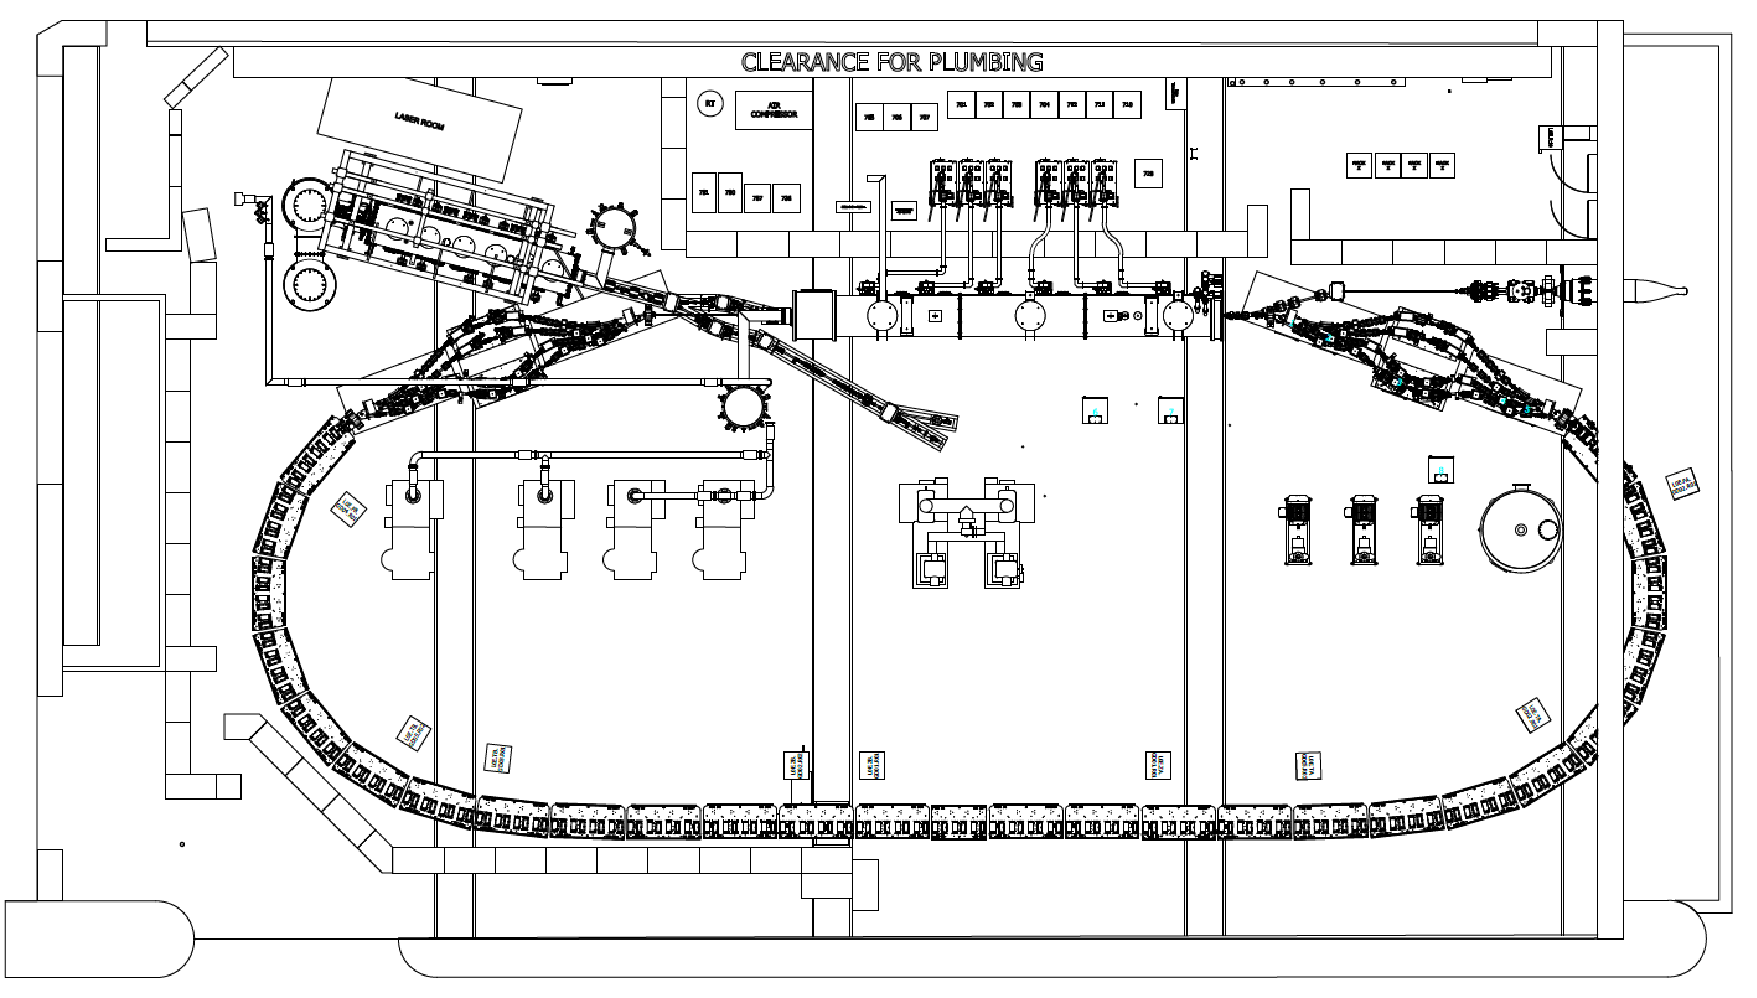
\includegraphics[width=0.8\textwidth]{Figures/CBETA_Inverse_Compton_Source_Design/CBETA_schematic.pdf}
\caption{Schematic of the CBETA ERL; existing accelerator structure including injector, main linac cryomodule, FFAG return loop, splitter and recombiner systems and beam dump, as well as supporting infrastructure such as electronic racks, vaccuum pumps and shielding. \textcolor{blue}{Who do I reference for this? Ask Kirsten!}}
\label{fig:CBETA_schematic}
\end{figure}

The layout of such a bypass line is shown in Fig.~\ref{fig:CBETA_ICS_Layout}. The bypass is configured for 150~\si{\mega\electronvolt} 4th-pass operation but could be adapted to operate with all nominal energies. The bypass was designed and optimised using the \textsc{Bmad} accelerator simulation library~\cite{BmadManual} and the \textsc{Tao} program~\cite{TaoManual} for simulating high
energy particle beams in accelerators.

%\textcolor{blue}{\begin{itemize}
%    \item{In different plane from CBETA}
%    \item{IP in different plane from CBETA and bypass}
%    \item{$\beta$-functions at the IP tunable between the baseline and optimised values}
%    \item{$\alpha_{x/y} =0$, $\eta_{x/y} =0$, $\eta'_{x/y} =0$ at the IP in each case}
%    \item{Path length tunability $\pm \lambda_{\mathrm{RF}}$}
%    \item{$R_{56} = 0$ for 5th linac pass, as this is the value for standard 5th pass.}
%    \item{Small peak $\beta$-functions and dispersion throughout the lattice - sensitivity issues}
%\end{itemize}}

\begin{figure}[!h]
\centering
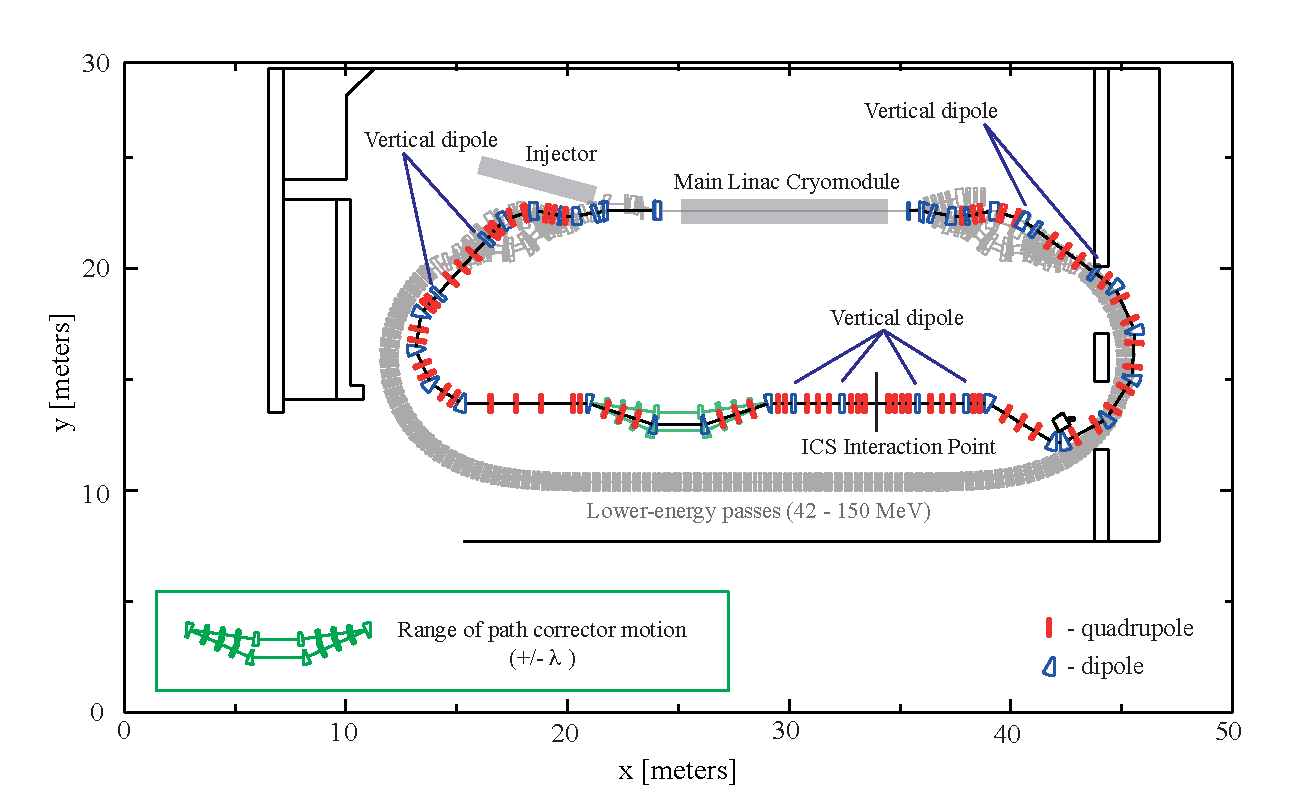
\includegraphics[width=0.8\textwidth]{Figures/CBETA_Inverse_Compton_Source_Design/cbetaicslayout.pdf}
\caption{Layout of the ICS bypass in CBETA; greyed beamline elements are already installed in the existing accelerator. Outer walls and relevant existing infrastructure shown in black.}
\label{fig:CBETA_ICS_Layout}
\end{figure}

The bypass line diverts the 150~\si{\mega\electronvolt} electron beam after the 4th linac pass in the corresponding S4 splitter line; the electron beam then re-enters the existing layout in the R4 line. The bypass replaces the FFA return loop, S4, from the 4th dipole onward and R4 up to the 4th dipole. The bypass will be located above the existing permanent magnet arc as the FFA arc is still used to transport the lower energy (42, 78, and 114~MeV) beams before and after the bypass.

A system of vertical doglegs, replacing sections of the S4 and R4 lines, are required to provide a 30~\si{\centi\meter} vertical elevation of the bypass line relative to the plane of the FFA return loop in order to avoid the existing accelerator. Single step vertical doglegs are preferred over the staircase style vertical doglegs used in the CEBAF spreader \cite{york1987optics}, as they offer a smaller footprint; desirable in a compact accelerator. However, this comes at the cost of increased dispersion growth and therefore poor $R_{56}$. Increased dispersion growth can be mitigated by additional focusing though in the CBETA case additional focusing is not required as the vertical doglegs are short enough to limit the impact on $R_{56}$.   
Bypass arc sections replace the existing FFA arc sections (FA, FB). Following the first arc, there is a horizontal dogleg used to close horizontal dispersion before the interaction region and offset the bypass from existing infrastructure. 

At the interaction region (IR) the beam is again offset upward locally by a further 20~\si{\centi\meter} -- to a 50~\si{\centi\meter} total offset above the FFA reference orbit height -- using a pair of vertical doglegs; these are here called the IR doglegs. The further vertical offset is imposed so the photons are produced in a different plane to both the bypass line and FFA return loop which is necessary for the extraction of the x-ray beam to an external experimental hutch and in order to avoid irradiation of the FFA permanent magnets. \textcolor{blue}{**TALK ABOUT POTENTIAL EXPERIMENTAL HUTCH POSITION**} A flexible focusing section within the pair of IR doglegs is used to focus to the required beam waist. The final focus section is designed to enable both $\beta^{*} = 1$~\si{\centi\meter} for the baseline case and $\beta^{*} = 12.6$~\si{\centi\meter} for the 0.5\% \textit{rms} bandwidth case (see Table~\ref{tab:CBETA_electron_beam_design_parameters}). Further interaction point conditions require $\alpha_{x/y} =0$ and the dispersion and it's derivative be zeroed ($\eta_{x/y} = 0$, $\eta'_{x/y} = 0$). \textcolor{blue}{**WHY?**} The final focus section is based on a low $\beta$ insertion \cite{chao2013handbook} and is constructed from 7 quadrupoles with the laser re-circulation cavity placed between the 4th and 5th quadrupole. Quadrupole triplets are used to focus the bunch to the required small waist for interaction whilst the 7th IR quadrupole is used to aid matching of the outgoing interaction vertical dogleg. This scheme allows the photons to be extracted via the first dipole of the downstream IR dogleg, minimizing the number of magnets requiring modification for photon extraction. 

\textcolor{blue}{**NEEDS WORK**}

Within the straight section of the bypass following the IR, variable path length adjustment is implemented based on the moving chicane described by H. Owen et al~\cite{owen2012modular}; this 4-dipole focusing chicane uses two mechanically-adjustable swing arms each incorporating a quadrupole triplet, and a central bellows. 

For the 4th pass of CBETA, the total path length must be altered by $(n+1/2)\lambda_{\mathrm{RF}}$ so the electron beam is decelerated in the subsequent pass. Small adjustments are typically made to the path length by the splitter/recombiner lines, however in the bypass design these have been bisected and  can not accomplish this task. 

The chicane replicates the function of the S4/R4 splitter/recombiners to allow variation of both $R_{56}$ and path length for re-entry into the MLC.  Path length adjustment is made by opening the swing arms of the chicane whilst increasing the dipole strengths accordingly. With this system a path length adjustment of $\pm\lambda_{\mathrm{RF}}$ is possible, which corresponds to 180\si{\degree} of linac phase; more than adequate for adjustment of the bypass line. Over a change in path length of $\pm\lambda_{\mathrm{RF}}$ the variation in Twiss values (after re-matching) is moderate, as can be seen in Figure~\ref{fig:CBETA_ICS_Twiss}.

\textcolor{blue}{**TALK ABOUT 2nd ARC, VERTICAL DOGLEG + MERGE TO 5th LINAC PASS + MATCHING CONDITIONS**}

The quality of the Twiss parameter matching of the bypass is limited by the compact layout of CBETA, the conditions required for energy recovery of the interacted beam, re-entry from the bypass to the 5th linac pass (Twiss matching, $R_{56} =0$), and the necessity for the bypass to be constructed above the existing FFA return loop; the $\beta$-functions and dispersion remain feasible. Plots of $\beta$-functions and dispersion in the bypass line for the 0.5\% \textit{rms} bandwidth case are shown in Figs.~\ref{fig:CBETA_ICS_Twiss} and~\ref{fig:CBETA_ICS_dispersion}. 

\begin{figure}[!h]
    \centering
    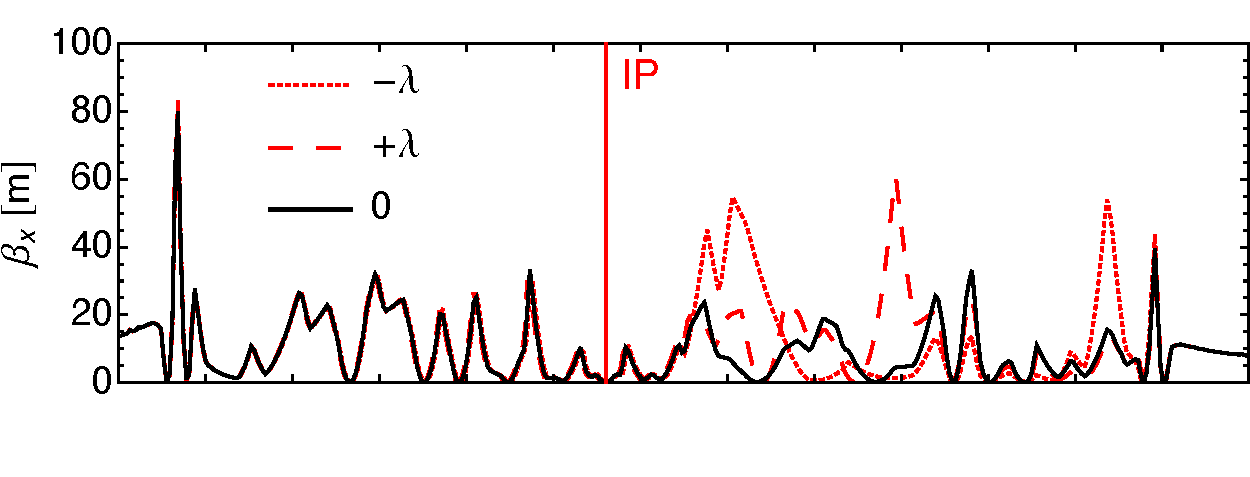
\includegraphics[width=0.5\textwidth]{Figures/CBETA_Inverse_Compton_Source_Design/twissplotx.pdf}
    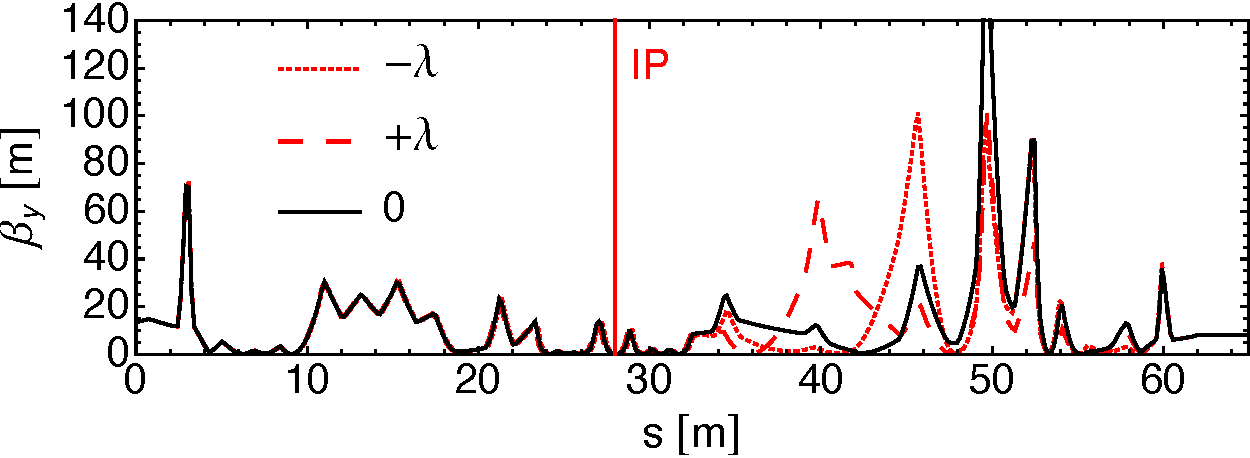
\includegraphics[width=0.5\textwidth]{Figures/CBETA_Inverse_Compton_Source_Design/twissploty.pdf}
    \caption{Twiss functions in the ICS bypass line, showing the re-matched conditions for different path length configurations $-\lambda_{\mathrm{RF}}$, $0$ and $+\lambda_{\mathrm{RF}}$. The ICS interaction point (IP) is indicated. \textcolor{blue}{Potentially worth putting the beta functions and dispersion functions side by side?}}
    \label{fig:CBETA_ICS_Twiss}
\end{figure}

\begin{figure}[!h]
\centering
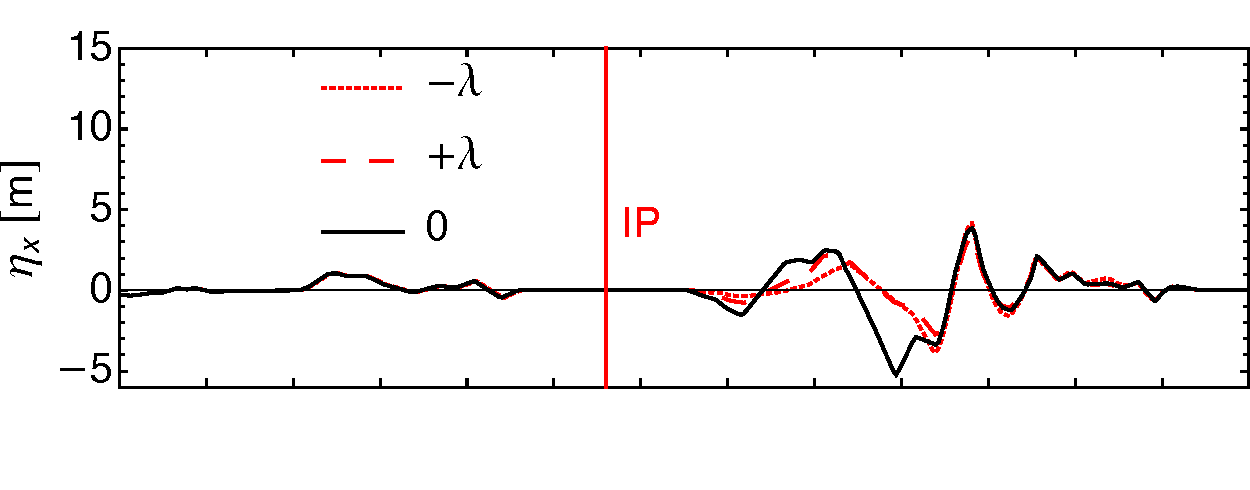
\includegraphics[width=0.5\textwidth]{Figures/CBETA_Inverse_Compton_Source_Design/dispplotx.pdf}
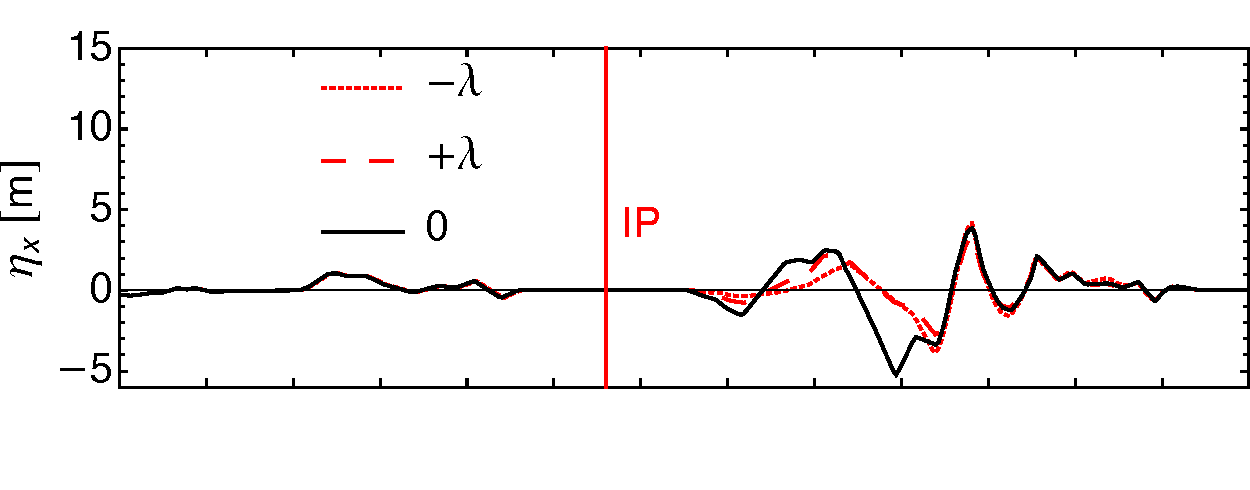
\includegraphics[width=0.5\textwidth]{Figures/CBETA_Inverse_Compton_Source_Design/dispplotx.pdf}
\caption{Dispersion functions in the ICS bypass line for the 0.5\% \textit{rms} bandwidth case, showing the re-matched conditions for different path length configurations $-\lambda_{RF}$, $0$ and $+\lambda_{RF}$. The ICS interaction point (IP) is indicated.}
\label{fig:CBETA_ICS_dispersion}
\end{figure}

The solution for the 150~\si{\mega\electronvolt} 4th pass could be generalised to the lower energy passes to form configurable ICS sources from each line. Electron bunches would be re-routed through the S4 line, magnet strengths would be scaled and re-matched, the optimised IP focusing solution for each line, as in Table~\ref{tab:CBETA_electron_beam_design_parameters} would be adhered to, and the path length correction system demonstrates the necessary flexibility for $\pm\lambda_{RF}$ adjustment which would be sufficient.

The 150~\si{\mega\electronvolt} nominal energy is potentially the most challenging as this requires the highest gradient magnets for focusing at the IP, path length correction and transport. However, in standard 4-pass operation this transport line is only traversed once, each other line is traversed twice in both acceleration and deceleration configuration.

For example, the 3rd pass 114~\si{\mega\electronvolt} nominal energy transport line is traversed on both the 3rd turn (accelerating pass) and the 5th turn (decelerating pass). If the ERL is still operated in 4-pass mode, the bypass line (for the 3rd pass) has to satisfy both sets of conditions imposed on the accelerating and decelerating pass whilst maintaining the same IP focusing constraints. The electron bunch must be delivered to the IP with the same longitudinal and transverse profile or consecutive electron bunch--photon pulse interactions will produce radiation with varying spectral characteristics. Alternatively, the ERL could be operated as a 3-pass ERL for the purpose of an ICS at the 3rd nominal energy. A decelerating configuration bunch is interacted at the IP meaning the produced radiation is identical for each interaction. Sufficient flexibility would be required within this bypass line as decelerating pass linac matching condition require replication and a 180$\degree$ phase change  is compulsory, irrespective of electron kinetic energy. There would also be consequences for repetition rate of the ICS interaction.   

\textcolor{blue}{**NEEDS A BIT OF WORK THIS, EXPLAIN BETTER**}

The author favours the latter solution to this problem as common transport systems in ERLs are already typically highly constrained - more-so for the FFAG multiple energy common transport system in CBETA  (\textcolor{blue}{reference to the relevant part in CBETA ERL commissioning}) - and the latter solution appears to offer less constraints on the beam dynamics. Of course, this issue could be avoided entirely via the use of single transport, where we have different transport beamlines for both the accelerating and decelerating configuration of each nominal energy of the multi-turn ERL, with ICS interaction points integrated, not retrofitted into the design.     

\textcolor{blue}{**BYPASS TRACKING STUDIES**}

\section{Spectral Output}

In order to determine the performance of the CBETA inverse Compton scattering source, the predicted spectral output of the source -- several measures quantifying the output radiation -- must be characterised using the formulae in Chapter~\ref{Photon_Production_by_Inverse_Compton_Scattering}. Anticipated spectral output of the CBETA inverse Compton scattering source is denoted in Table~\ref{tab:CBETA_spectral_output}, where the baseline and the 0.5\% \textit{rms} bandwidth optimised configurations are both shown. 

\textcolor{blue}{**WHAT IS THE OPTIMISED CONFIGURATION, HOW IS IT ACHIEVED + WHY IS IT CHOSEN FOR CBETA ICS**}
The optimised configuration has been achieved using the 

\begin{table}[!h]
\caption{Anticipated photon output for each of the four electron beam energies in CBETA, taking into account a 5~degree crossing angle. The recoil parameter is negligible $X < 0.003$, even at  150~MeV -- the maximum electron beam energy. The collimated flux has been optimised for a 0.5\% \textit{rms} bandwidth and the baseline case focuses at the IP to $\beta^{*} =1$~\si{\centi\meter} for each nominal energy.}
\scalebox{0.92}{
\begin{tabular}{lccccc}
\hline\hline
 & \multicolumn{4}{c}{Electron Kinetic Energy (\si{\mega\electronvolt})} & \\
 \cline{2-5}
 & 42 & 78 & 114 & 150 & \\
\hline
X-ray peak energy & 32.2 & 109.7 & 233.1 & 402.5 & \si{\kilo\electronvolt}\\
Source Size & 5.84 & 4.35 & 3.62 & 3.17 & \si{\micro\meter} \\
Uncollimated flux & 3.16$\times10^{10}$ & 3.20$\times10^{10}$ & 3.21$\times10^{10}$ & 3.22$\times10^{10}$ & ph/\si{\second}\\
Spectral density & 9.82$\times10^{5}$ & 2.92$\times10^{5}$ & 1.38$\times10^{5}$ & 8.00$\times10^{4}$ & ph/\si{\second} \second{\electronvolt}\\
Average brilliance & 9.23$\times10^{10}$ & 3.19$\times10^{11}$ & 6.81$\times 10^{11}$ & 1.18$\times10^{12}$ & ph/\si{\second} \si{\milli\meter}$^{2}$-\si{\milli\radian}$^{2}$ 0.1\% bw\\
Peak brilliance & 2.80$\times 10^{15}$ & 1.00$\times 10^{16}$ & 2.18$\times10^{16}$ & 3.80$\times 10^{16}$ & ph/\si{\second} \si{\milli\meter}$^{2}$-\si{\milli\radian}$^{2}$ 0.1\% bw\\
\hline
 & \multicolumn{4}{c}{0.5\% \textit{rms} bandwidth} & \\
\hline
Source Size & 10.25 & 10.34 & 10.32 & 10.35 & \si{\micro\meter} \\
Collimated flux & 2.09$\times 10^{8}$ & 2.09$\times 10^{8}$ & 2.09$\times 10^{8}$ & 2.09$\times 10^{8}$ & ph/\si{\second} 0.5\% bw \\
\hline\hline
\end{tabular}}
\label{tab:CBETA_spectral_output}
\end{table}

\textcolor{blue}{**DECIDE WHICH OPTIMISATION METHOD TO SHOW IN THE TABLES** \\ **USE NEW PEAK BRILLIANCE**}

We can see from Table~\ref{tab:CBETA_spectral_output} that uncollimated flux varies by around 2\% due to the small effect of the electron spot size. Recoil effects are negligible even at the highest electron beam energy $E_{e} = 150$~\si{\mega\electronvolt}, as $X = 2.70\times 10^{-3}$.  

The number of scattered photons is essentially independent of electron energy for a fixed electron spot size at the IP, and since both the Compton spectrum and the (relative) 0.5\% \textit{rms} bandwidth scale together with $\gamma^2$, both the optimised spot size and the predicted collimated fluxes are the same at all electron energies.

From Table~\ref{tab:CBETA_laser_pulse_design_parameters}, we see this deign incorporates a 5\si{\degree} crossing angle of the laser pulse with respect to the electron bunch which is necessary because of the Fabry-Perot optical cavity. The crossing angle causes only a $\sim 1$~\si{\kilo\electronvolt} reduction in the Compton edge scattered photon energy in comparison to the head-on case ($\phi = 0$). However, the crossing angle impacts the flux of the source significantly as the effective time over which the incident laser photons may interact with the electrons in the counter propagating bunch is reduced. This results in a factor of 5.5 reduction in luminosity due to a 5\si{\degree} crossing (Eq.~\ref{eq:angular_crossing_factor}) -- a substantial reduction in flux. 

The scattered photon energy of the source in independent of the hourglass effect. The hourglass does impact upon the luminosity of the source and therefore the flux is non negligible; the hourglass effect luminosity reduction (Eq.~\ref{eq:furman_hourglass_reduction}) is $R_{HG} = 0.96$, a 4\% reduction in flux for a head-on back-scattering arrangement. However, here we have both angular crossing and hourglass effect affecting the ICS source so we must use the full reduction factor (Eq.~\ref{eq:miyahara_combined_reduction}), resulting in a factor 5.57 reduction. This is near-identical to the angular crossing reduction factor as the hourglass effect is suppressed by the reduction in interaction time of the electron bunch and laser pulse. 

Table~\ref{tab:CBETA_spectral_output} also shows the brilliance of the source, both peak and average, increasing with nominal energy due to the $\mathcal{B} \propto \gamma^{2}$ relationship. Similarly, the spectral density decreases approximately inversely proportional to the Lorentz factor of the electron beam ($S \propto \frac{1}{\gamma^{2}}$). The two relations are approximate as they both also depend on flux, where we see a 2\% increase in collimated flux due to the aforementioned spot size effect. 

By applying the collimated flux maximisation to the parameter space of the round beam optimisation in Section~\ref{sec:RB_optimisation}, as shown in Fig.~\ref{fig:CBETA_beta_theta_parameter_space}, the collimated flux - \textit{rms} bandwidth tuning curve of the CBETA ICS within the 0--1\% \textit{rms} bandwidth range can be discerned, as shown in Fig.~\ref{fig:CBETA_Tuning_Curve}. 
\begin{figure}[!h]
\centering
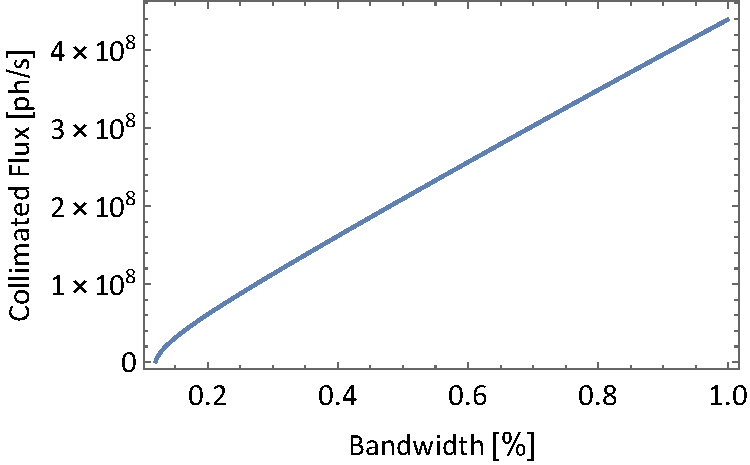
\includegraphics[width=0.7\textwidth]{Figures/CBETA_Inverse_Compton_Source_Design/CBETATuningCurve.pdf}
\caption{Tuning curve of collimated flux against \textit{rms} bandwidth for a 0--1\% \textit{rms} bandwidth range, produced by a round beam optimisation which tunes $\beta^{*}$ and $\theta_{\mathrm{col}}$. The tuning curve is independent of beam energy for scattering scenarios within the Thomson regime, hence this tuning curve applies to all energies in CBETA. The left end of tuning curve indicates the minimum possible \textit{rms} bandwidth of the ICS source, which in CBETA is $\simeq$~0.12\% and is determined by the electron beam and laser pulse energy spreads. \textcolor{blue}{**x-axis label needs to read \textit{rms} bandwidth**}}
\label{fig:CBETA_Tuning_Curve}
\end{figure}

In Fig.~\ref{fig:CBETA_Tuning_Curve}, the round beam optimisation tuning curves of the four nominal energies of the CBETA ICS are shown as a single line. This is as the recoil parameter for the CBETA ICS is near-negligible for the nominal operating energies of CBETA, which means the tuning curves directly overlap. The relationship between collimated flux and bandwidth for the CBETA ICS is linear past the rapid fall off at low bandwidth which is occurs once we approach the minimum theoretical limit of the bandwidth. Within the non-linear portion of Fig.~\ref{fig:CBETA_Tuning_Curve}, the energy spreads of the electron bunch and laser pulse dominate the bandwidth, which restricts the round beam $\beta^{*}$-$\theta_{\mathrm{col}}$ parameter space. Consequently the optimum balance between the emittance and collimation term can not be achieved, causing a rapid decrease in the collimated flux.
\textcolor{blue}{**EXPLAIN THE ENERGY DEPENDENCE OF THIS**}


\textcolor{blue}{**WRITE ABOUT THE SPECTRUM CODES A BIT + LINK TO THAT CHAPTER** \\ **WHAT AM I SHOWING HERE?**}

The spectrum of the scattered x-rays produced from a single head-on ($\phi = 0$) interaction of an electron bunch and laser pulse, collimated downstream into a 0.5\% \textit{rms} bandwidth for the 150~\si{\mega\electronvolt} is shown in Fig.~\ref{fig:CBETA_spectrum_benchmarking}. The spectrum here is produced using two individual semi-analytical spectrum codes: \textsc{ICARUS}, the development of which is covered in Section~\ref{sec:development_of_the_ICARUS_spectrum_code}, and \textsc{ICCS3D} \cite{krafft2016laser,ranjan2018simulation}. The \textsc{ICARUS} spectrum is produced using Gaussian models for the electron bunch and laser pulse whereas \textsc{ICCS3D} uses a Gaussian electron bunch model that has been tracked using \textsc{Tao} through CBETA ICS bypass, as detailed in Section~\ref{sec:bypass_design}, to the interaction point. Both codes operate for a head-on interaction, take into account the recoil effect, account for emittance in both transverse planes, model the effect of energy spread of the electron bunch and laser pulse (spectral bandwidth) and are capable of simulating both square and circular collimation. The CBETA ICS \textsc{ICARUS} and \textsc{ICCS3D} spectra show strong agreement as observed during the bench-marking in Section~\ref{sec:benchmarking_of_the_ICARUS_spectrum_code}.

\begin{figure}[!h]
\centering
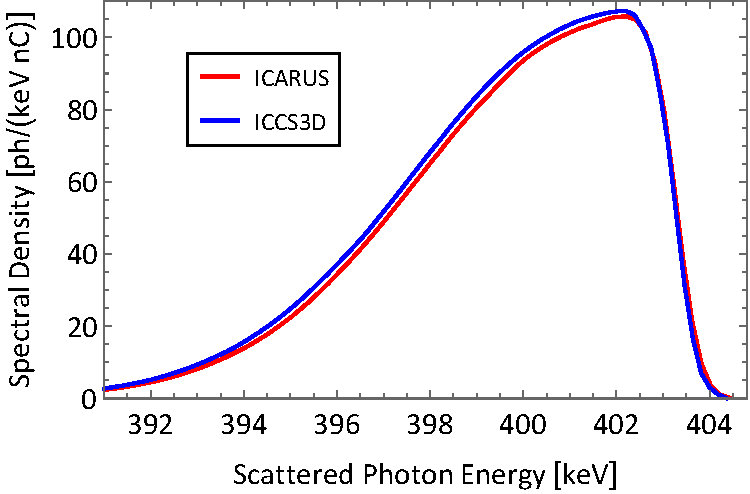
\includegraphics[width=0.8\textwidth]{Figures/CBETA_Inverse_Compton_Source_Design/cbetaspectrumplot_final.pdf}
\caption{Predicted spectral output (flux) from 1064~\si{\nano\meter} photons colliding head-on with the $E_e =150$~\si{\mega\electronvolt} (kinetic energy) electrons in CBETA; this spectrum was generated using the \textsc{ICCS3D} and \textsc{ICARUS} codes. This spectrum has a peak energy of 403.3~\si{\kilo\electronvolt}; using the proposed 5\si{\degree} crossing angle, the peak energy is reduced to 402.5~\si{\kilo\electronvolt} and the spectral density is reduced by a factor $\sim$~6.}
\label{fig:CBETA_spectrum_benchmarking}
\end{figure}

In Fig.~\ref{fig:CBETA_spectrum_benchmarking} the case of the CBETA ICS at 150~\si{\mega\electronvolt} is shown with a peak photon energy of 403.3~\si{\kilo\electronvolt}, 0.8~\si{\kilo\electronvolt} above the value shown in Table~\ref{tab:CBETA_spectral_output} because this is for the head-on case. 

We see that the maximum photon energy is higher than the predicted Compton edge energy at $\sim$~405~\si{\kilo\electronvolt}, this is because of the energy spread of the electron bunch and the spectral bandwidth of the laser pulse mean that an incident electron or photon can have a higher energy photon that the nominal energy and therefore generate a photon beyond the expected peak energy of the Compton edge. This phenomena also explains why the spectrum isn't hard edged but is smoothed around the peak scattered photon energy of the spectrum. 

The spectral density of the spectrum is truncated due to the collimator. However, the various optimisation procedures detailed in Chapter~\ref{Optimisation_and_Characterisation_of_Inverse_Compton Scattering_Spectra} are designed to mitigate this effect. The collimation is also crucial in providing the specified \textit{rms} bandwidth due to the scattered photon energy--scattering angle correspondance ($E_{\gamma}\propto\theta$) . The effect of emittance in the spectrum is directly observable in the long tails of the spectrum, the transverse emittance of the electron bunch varies the divergence of the scattered radiation and therefore allows lower energy photons to pass through the collimator. 

\section{X-ray ICS Source Comparison}
\label{sec:xray_ICS_comparison}

Many inverse Compton scattering sources driven by a variety of accelerator types have been designed and built to operate in the x-ray regime, the CBETA ICS can be compared against these to evaluate the quality of the ERL driven ICS approach. Direct comparison is difficult as different designs have different objectives -- one design may prioritize maximizing flux while another prioritizes having a narrower bandwidth.

To collate ICS sources of interest, we arbitrarily limit our discussions to the scattered photon energy range $1$~\si{\kilo\electronvolt} ($\sim$10~\si{\angstrom}) $< E_{\gamma} <$ 1~\si{\mega\electronvolt} ($\sim$0.01~\si{\angstrom}). A survey of x-ray inverse Compton sources is presented in Table~\ref{tab:xray_ICS_comparison}.

\begin{table}[!h]
\caption{Comparison of existing and designed x-ray ICS.}
\begin{threeparttable}
\begin{tabular}{lccc}
\hline\hline
ICS & Accelerator Type & Scattered Photon Energy (\si{\kilo\electronvolt}) & Flux (ph/\si{\second}) \\
\hline
cERL \cite{akagi2016narrow} & ERL & 6.95 & 2.6$\times 10^{7}$ \\ 
ALICE \cite{priebe2008inverse,priebe2010first} & ERL & 21.5 & 9$\times 10^{5}$ \\
MIT ICS\tnote{*} ~\cite{graves2014compact} & Linac & 3 - 30 & 3$\times 10^{14}$ \\
MuCLS \cite{eggl2016munich} & Storage Ring & 15 - 35 & 0.443 - 1.78$\times 10^{10}$ \\ 
Tsinghua \cite{du2013generation} & Linac & 51.7 & 1$\times 10^{6}$ \\
ThomX\tnote{*} ~\cite{variola2014thomx,dupraz2020thomx} & Storage Ring & 45 - 90 & $1\times 10^{10}$ - $10^{13}$ \\
BriXS\tnote{*} ~\cite{faillace2019status,drebot2019brixs,cardarelli2020brixs} & ERL & 20 - 180 & $1\times 10^{10}$ - $10^{13}$ \\
CBETA\tnote{*} & ERL & 32.2, 109.7, 233.1, 402.5 & 3.16 - 3.21$\times 10^{10}$ \\ 
NIJI-IV \cite{sei2017demonstration} & Storage Ring & 1200 & 3.1$\times 10^{4}$ \\ 
HI$\gamma$S\tnote{$\dagger$} ~\cite{weller2009research} & Storage Ring & 1000 - 3000 & 5$\times 10^{7}$ - 5$\times 10^{8}$ \\
\hline\hline
\end{tabular}
\begin{tablenotes}
\item[*]{Denotes design parameters for sources which are not yet demonstrated.}
\item[$\dagger$]{The HI$\gamma$S source is capable of scattered photon energies up to 100~\si{\mega\electronvolt}. Shown is the lowest energy operational setting.}
\end{tablenotes}
\end{threeparttable}
\label{tab:xray_ICS_comparison}
\end{table}

As evident from Table~\ref{tab:xray_ICS_comparison}, the 3rd and 4th pass ICS sources on CBETA nopminally produce x-rays at 233~\si{\kilo\electronvolt} and 403~\si{\kilo\electronvolt} respectively. Therefore, these offer unparalleled access to the $< 200$~\si{\kilo\electronvolt} x-ray regime, enabling a series of new high energy x-ray applications as shown in Section~\ref{sec:CBETA_ICS_applications}.

The highest flux x-ray ICS demonstration is the 1.78$\times 10^{10}$~ph/\si{\second} demonstration at MuCLS \cite{eggl2016munich}, which uses a small ($\sim4$~\si{\meter} diameter) storage ring and a 70~\si{\kilo\watt} average stored power Fabry-Perot optical cavity. The CBETA ICS source design excels this by a factor $\sim2$. However, CBETA ICS is also capable of a much smaller bandwidth due to the smaller energy spread of the ERL in comparison with a storage ring.

The CBETA ICS design outclasses the cERL ICS demonstration, the highest flux ERL driven ICS source, in terms of flux by a factor of $\sim1000$. As the Fabry-Perot optical cavity for CBETA is based upon the cERL ICS design, the difference is mainly due to the increase in bunch charge of CBETA in comparison to cERL (32~\si{\pico\coulomb} $>$ 0.355~\si{\pico\coulomb}) and the smaller electron bunch spot size at the interaction point (for the baseline case).

The design of the BriXS and ThomX ICS sources offer fluxes up to $10^{13}$~ph/\si{\second} which are a factor $\sim300$ higher than those predicted for the CBETA ICS. In the BriXS case this is because the push-pull ERL design expects a much higher bunch charge than CBETA (32~\si{\pico\coulomb} < 200~\si{\pico\coulomb}) \cite{drebot2019brixs} and the average stored power at 750~\si{\kilo\watt} \cite{drebot2019brixs} is greater than the 670~\si{\kilo\watt} highest average stored power demonstration \cite{carstens2014megawatt} outside of an accelerator environment. The ThomX source intends to increase its flux in three steps corresponding to bunch charges of 50~\si{\pico\coulomb}, 100~\si{\pico\coulomb} and 1~\si{\nano\coulomb} with average stored powers in the Fabry-Perot cavity of 100~\si{\kilo\watt}, 500~\si{\kilo\watt} and 1~\si{\mega\watt} with the repetition rate being increased a factor of 5 from the first to second stage \cite{dupraz2020thomx}. These parameter sets lead to predicted fluxes of $10^{11}$~ph/\si{\second}, $10^{11}$~ph/\si{\second} and $10^{13}$~ph/\si{\second}. However, a Fabry-Perot optical cavity beyond the 70~\si{\kilo\watt} average stored power demonstration of MuCLS \cite{eggl2016munich} has not been shown to be operable as part of an ICS source. When the ThomX source parameters are within the state-of-the-art, the flux is comparable to that of the CBETA ICS.   

% MIT ICS a special case - why?

\section{Synchrotron Facility Comparison}
\label{sec:synchrotron_facility_comparison}

% review of how x-rays can be produced
% why is synchrotron the main competitior
% mention SRS + Ian Munro @ Daresbury

Inverse Compton production of photons at CBETA has the ability to extend the reach of monochromatic photon sources toward \si{\mega\electronvolt} scale, as shown in Table~\ref{tab:CBETA_spectral_output}. Alternative sources are bremsstrahlung methods, though these generate intrinsically broad-band radiation, line sources such as $^{137}$Cs and $^{60}$Co, and synchrotron radiation. Whilst line sources provide photons in the \si{\mega\electronvolt} scale, they are not tuneable, emit isotropically and require proper handling. Therefore, synchrotron radiation sources such as undulators are currently the premier method to generate intense, narrow-band radiation tunable on a \si{\kilo\electronvolt} to \si{\mega\electronvolt} scale. Hence, evaluation of the CBETA ICS as a source of monochromatic x-ray radiation is best attained by direct comparison with leading synchrotron radiation sources as well as other inverse Compton scattering sources (Section~\ref{sec:xray_ICS_comparison}).   

Krafft and Priebe \cite{krafft2010compton} hypothesised that flux and brilliance offered by ICS sources is not competitive at the photon energies produced by 3rd generation light sources such as synchrotron radiation facilities. Subsequently, recent x-ray ICS source designs are intended to compromise between typical labratory-scale sources, such as synchrotron radiaton facilities and rotating cathode tubes,in terms of size, cost, access, availability, and x-ray quality \cite{deitrick2018high}. \textcolor{blue}{- would be nice to re-arrange this so we delineate the weak points of each of these}.
The CBETA ICS source design provides scope to test Krafft and Priebe's hypothesis because it spans to the 100's~\si{\kilo\electronvolt} regime which allows better assessment of the utility of ICS production at the limits of synchrotron production.

The characteristic critical photon energy for synchrotron radiation is
\begin{equation}
\epsilon_{c}=\frac{3}{2}\frac{\hbar c \gamma^3}{\rho},
\label{eq:synchrotron_critical_energy}
\end{equation}
which can be recast in more natural units as $\epsilon_{c}$[\si{\kilo\electronvolt}]$\simeq 0.665E^{2}B$ (for $E$, the electron kinetic energy, given in \si{\giga\electronvolt} and $B$, the magnetic flux density of the bending magnets, in \si{\tesla}). The highest-energy 3rd-generation light source source today is SPring-8 with $E = 8$~\si{\giga\electronvolt} and $B\simeq 0.68$~\si{\tesla} to obtain a critical energy $\epsilon_{c}\simeq 29$~\si{\kilo\electronvolt} for its broadband incoherent SR production. Storage rings for 3rd generation light sources, such as SPring-8, have a physical circumference exceeding 1~\si{\kilo\meter} therefore due to financial considerations it is unlikely that a storage ring above 8~\si{\giga\electronvolt} will be built. 

The undulator output limit from a storage ring can be illustrated by setting the undulator $K$-parameter to be $K \sim 1$ and an undulator period $\lambda_u \sim$~1~\si{\centi\meter}. This gives a magnetic field limit of
\begin{equation}
B_0 = \frac{m_{e} c}{e}\frac{2\pi}{\lambda_{u}} K \simeq 1\textrm{T}.
\label{eq:undulator_field_limit}
\end{equation}
The minimum undulator wavelength ($K=0$) possible (in the fundamental harmonic of emission) is
\begin{equation}
\lambda_\textrm{min} = \frac{\lambda_{u}}{2 \gamma^2} \simeq 0.2 \textrm{\AA}
\label{eq:undulator_minimum_wavelength}
\end{equation}
at 8~\si{\giga\electronvolt} ($\gamma \sim 15,700$), corresponding to a photon energy of $62$~\si{\kilo\electronvolt}. In practice, most hard x-ray undulators and wigglers operate up to around 100~\si{\kilo\electronvolt} photon energy by using higher harmonics, with few existing beamlines extending beyond that. Undulator output at higher harmonics is energy limited predominantly by the presence of magnetic phase errors, and the reduction factor $R$ in ideal flux from an \textit{rms} phase error $\sigma_{\phi}$ can be modelled approximately \cite{walker1993interference} using 
\begin{equation}
R=\exp{\left(-n^2 \sigma_{\phi}^{2}\right)},
\label{eq:undulator_phase_errors}
\end{equation}
where $n$ is an integer (odd) undulator harmonic number, and $\sigma_\phi$ typically has a value of a few degrees \cite{walker2013phase}. In practice this limits undulators to $n<15$ in operation, although there is still debate on the pessimism of the \textit{rms} error in some cases \cite{tanaka2018universal} and around schemes for reduction of $\sigma_{\phi}$ future insertion devices \cite{hwang2011development,huang2017challenges}.

Hard x-ray sources presently available at the high-energy storage rings APS \cite{apsbeamlines}, ESRF-EBS \cite{esrfbeamlines}, PETRA-III \cite{petraiiibeamlines}, and SPring-8 \cite{spring8beamlines}, have been surveyed. The codes \textsc{SPECTRA} \cite{tanaka2001spectra} and \textsc{SRW} \cite{chubar2013wavefront} are used to validate expected spectral output \cite{tanaka2001field}. For example, the flux of the SPring-8 BL10XU beamline  including a 5~\si{\degree} \textit{rms} phase error is shown in Fig.~\ref{fig:ICS_vs_SPRING8_Undulator_Flux}; this is compared with sample fluxes at the source points presented by SPring-8 \cite{spring8beamlines} and with the predicted flux from the CBETA ICS source design plotted as tabulated in Table~\ref{tab:CBETA_spectral_output}.

\begin{figure}[!h]
\centering
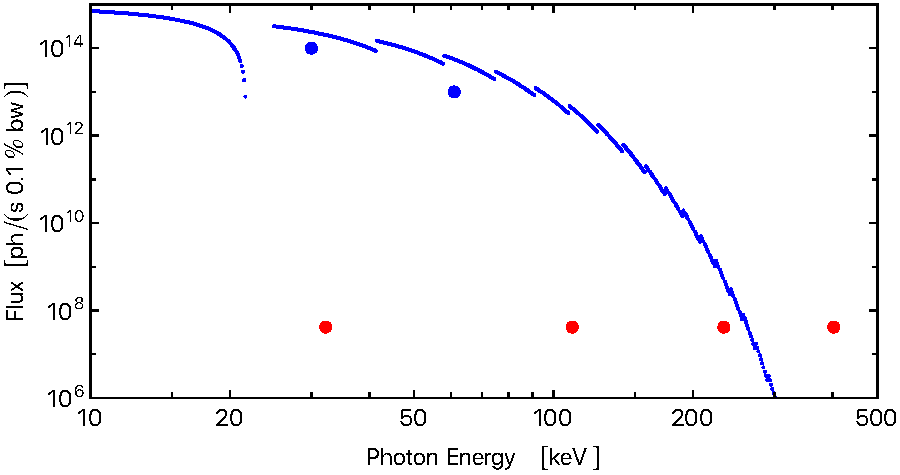
\includegraphics[width=0.8\textwidth]{Figures/CBETA_Inverse_Compton_Source_Design/spring8bl10fluxplot.pdf}
\caption{Comparison of CBETA predicted flux (here flux in a 0.1\% \textit{FWHM} bandwidth to allow comparison with conventional calculations of undulator flux) at the four discrete operating energies given in Table~\ref{tab:CBETA_spectral_output} with the output from a typical high-energy undulator. The undulator shown is the SPring-8 BL10XU insertion device~\cite{spring8beamlines} assuming an \textit{rms} phase error of 5\si{\degree}. Whilst this undulator is not designed to deliver good output at high harmonic number, it offers a useful guide to possible 3rd-generation source output in the 100~\si{\kilo\electronvolt} to 500~\si{\kilo\electronvolt} range. the measured flux at 30~\si{\kilo\electronvolt} and 61~\si{\kilo\electronvolt} for this beamline is also shown~\cite{spring8beamlines}. We predict that CBETA flux at 402~\si{\kilo\electronvolt} (150~\si{\mega\electronvolt} electron energy) exceeds that from 3rd-generation sources.}
\label{fig:ICS_vs_SPRING8_Undulator_Flux}
\end{figure}

The predicted brilliance of CBETA at the nominal energies of each turn energies is compared in Fig.~\ref{fig:ICS_vs_SPRING8_Undulator_Brilliance} with a high-energy undulator (BL10XU) at SPring-8 -- the worlds highest-energy 3rd-generation synchrotron source. Because the SPring-8 BL10XU undulator is not particularly atypical, Fig.~\ref{fig:ICS_vs_SPRING8_Undulator_Brilliance} is indicative of achievable brilliance from other state-of-the-art synchrotron facilities. This statement also holds for the flux case.

\begin{figure}[!h]
\centering
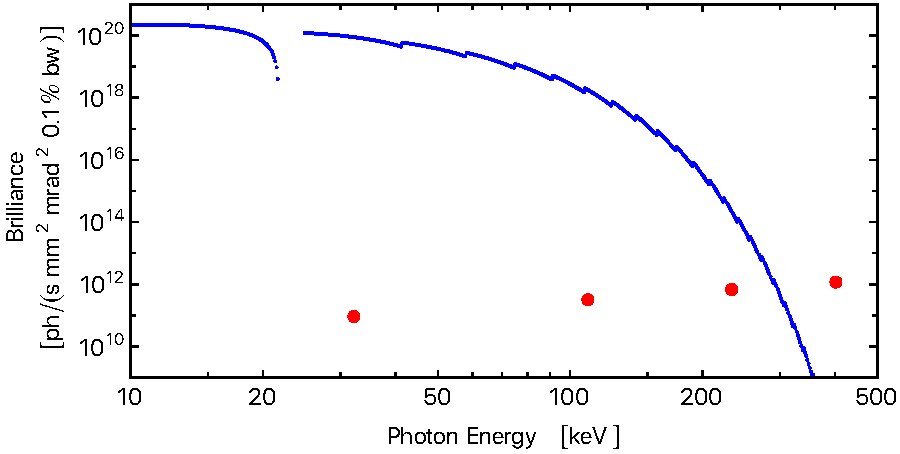
\includegraphics[width=0.8\textwidth]{Figures/CBETA_Inverse_Compton_Source_Design/spring8bl10brillianceplot.pdf}
\caption{Comparison of CBETA predicted brilliance at the four discrete operating energies given in Table~\ref{tab:CBETA_spectral_output} with the output from a typical high-energy undulator. The undulator shown is the SPring-8 BL10XU insertion device~\cite{spring8beamlines} assuming an \textit{rms} phase error of 5\si{\degrees}. We predict that CBETA brilliance at 402~\si{\kilo\electronvolt} (150~\si{\mega\electronvolt} electron kinetic energy) exceeds that from 3rd-generation sources.}
\label{fig:ICS_vs_SPRING8_Undulator_Brilliance}
\end{figure}

As hypothesized by Krafft and Priebe \cite{krafft2010compton}, storage ring sources produce greater brilliance and flux at high harmonic number for photon energies up to approximately 300~\si{\kilo\electronvolt}. However, the fundamental energy scaling of synchrotron radiation and the finite undulator magnetic field quality means that the ICS output from CBETA becomes superior beyond 300~\si{\kilo\electronvolt}. From Fig.~\ref{fig:ICS_vs_SPRING8_Undulator_Flux} we see the measured flux at 30~\si{\kilo\electronvolt} and 61~\si{\kilo\electronvolt} \cite{spring8beamlines} is orders of magnitude superior to that from an ICS source, but at 400~\si{\kilo\electronvolt} this is reversed. From inspection of other ICS source designs in Table~\ref{tab:xray_ICS_comparison} it is evident that ICS sources are projected to achieve $\sim 10^{10} - 10^{13}$~ph/\si{\second} independent of scattered photon energy so we can broaden our conclusions state that the interface between utility of ICS sources and 3rd generation light sources lies at $< 300$~\si{kilo\electronvolt}. Therefore, the hypothesis of Krafft and Priebe \cite{krafft2010compton} must be modified to note that ICS sources become competitive against synchrotron light sources at around 300~\si{\kilo\electronvolt}.  

\begin{figure}[!h]
\centering
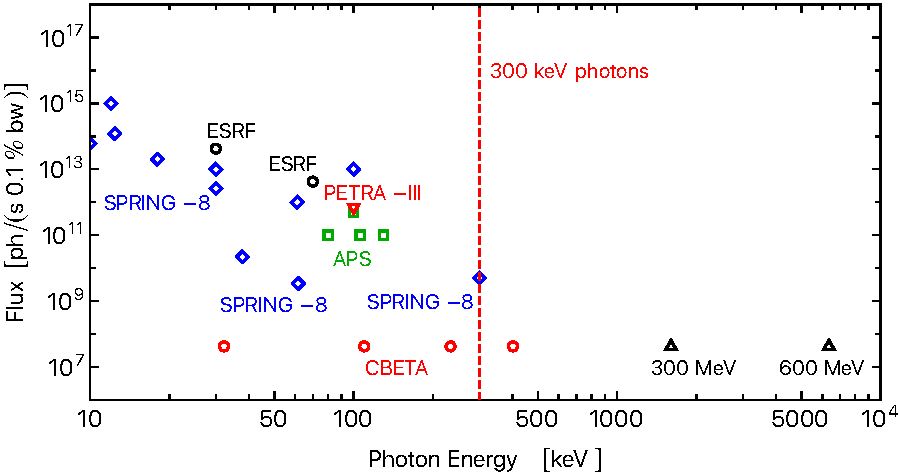
\includegraphics[width=0.8\textwidth]{Figures/CBETA_Inverse_Compton_Source_Design/sourcefluxcomparison.pdf}
\caption{On-sample measured fluxes from APS, ESRF-EBS, PETRA-III, and SPring-8 for which information has been published~\cite{apsbeamlines,esrfbeamlines,petraiiibeamlines,spring8beamlines}. This is compared with the predicted CBETA outputs in Table~\ref{tab:CBETA_spectral_output}, at the 4 discrete photon energies from 32 to 402~\si{\kilo\electronvolt}, and the predicted flux obtained by scaling the CBETA electron energy to 300~\si{\mega\electronvolt} (1.60~\si{\mega\electronvolt} photons) and 600~\si{\mega\electronvolt} (6.36~\si{\mega\electronvolt} photons). Whilst 3rd-generation sources are superior to ICS sources up to photon energies around 300~\si{\kilo\electronvolt}, they do not produce useable flux above 400~\si{\kilo\electronvolt}.}
\label{fig:ICS_Undulator_Comparison}
\end{figure}

Fig.~\ref{fig:ICS_Undulator_Comparison} compares the on-sample measured fluxes from those high-energy synchrotron beamlines ($>$30~\si{\kilo\electronvolt}) for which data is available \cite{apsbeamlines,esrfbeamlines,petraiiibeamlines,spring8beamlines}. Almost no beamline generates output above 100~\si{\kilo\electronvolt}, and above 300~\si{\kilo\electronvolt} we have shown that ICS is a superior production method. Extending the demonstrated CBETA parameters to higher electron energy we would expect the collimated flux values to remain nearly constant as we see that flux in inverse Compton scattering sources is broadly independent of electron kinetic energy. Hence we can estimate the likely possible flux for \si{\mega\electronvolt}-scale photons from a CBETA style ERL-based source. Therefore, two indicative electron energies (300~\si{\mega\electronvolt} and 600~\si{\mega\electronvolt}) are included in Fig.~\ref{fig:ICS_Undulator_Comparison}. The fluxes at 100's~\si{\mega\electronvolt}, based on a conservatively designed multi-pass ERL ICS, highlight the potential of this approach to $\gamma$-ray sources. 

\section{CBETA ICS Applications}
\label{sec:CBETA_ICS_applications}

The proposed CBETA ICS design provides a high-flux, small-bandwidth, quasi-monochromatic source of x-rays, producing high peak energy photons in the 100's~\si{\kilo\electronvolt} range. Large flux ($\sim 10^{10}$~ph/\si{\second}) at high energies ($< 100$~\si{\kilo\electronvolt}) opens up a parameter space for x-ray applications previously attainable only at the largest synchrotrons, and then only using substantial x-ray optics. Section~\ref{sec:synchrotron_facility_comparison} has shown that the CBETA ICS can achieve fluxes of $3.16\times 10^{10}$~ph/\si{\second} up to 402.5~\si{\kilo\electronvolt}, beyond that possible at a synchrotron radiation facilities therefore enabling new applications. Within this section an overview of the potential applications of the CBETA ICS are presented.   

\textcolor{blue}{**Minor section on removal of the necessity for x-ray optics due to energy--angle correspondence, or is this covered sufficiently elsewhere?**}

Photon beams produced by the CBETA ICS source could be used in important applications such as x-ray absorption spectroscopy (XAS) and x-ray fluorescence (XRF) \cite{willmott2019introduction}. High-energy XRF well-suited application for ICS sources as monochromation is not required, thereby avoiding complex x-ray optical instrumentation. Energy-sensitive x-ray fluorescence detection can be provided by a solid-state detector coupled to a pulse-height analyzer. For example, in analysis of a fission reactor's fuel rods, the $K\alpha$ and $K\beta$ lines for uranium ($K\alpha_{1} = 98.4$~\si{\kilo\electronvolt}, $K\beta_{1} = 111.3$~\si{\kilo\electronvolt}) and plutonium ($K\alpha_{1} = 103.7$~\si{\kilo\electronvolt}, $K\beta_{1} = 117.2$~\si{\kilo\electronvolt}) could be probed \cite{havrilla2015feasibility}. Quantitative assays and elemental determination would be performed through use of a low-$Z$ reference scatterer to ascertain the spectral content of the broadband incident beam via the elastic and Compton scattering into the same detector. Known energy dependent photo-absorption cross sections of the enable determination of the fluorescence efficiency of the detection scheme for elements of interest.

High energy photon production from the CBETA ICS source allows imaging of thick specimens as penetration depth of x-ray radiation scales with photon energy. The CBETA ICS could therefore be a prime tool to apply straightforward techniques such as 2D shadowgraphy through to more complex 3D reconstruction with tomography \cite{als2011elements} to thick samples. Due to the higher photon energies enabled by the CBETA ICS, this could extend the range of existing synchrotron radiation facilities.

Energy-dispersive x-ray diffraction (EDXRD), used for the identification of constituents of a poly-crystalline or powdered sample, is another application which exploits the high flux and high energy of the source. A high-flux source would allow for rapid identification of the minerals in a mined ore sample, while again the high energy of the source allows for the inspection of thick specimens. For commercial applications such as these the compact nature of the CBETA ICS is also advantageous. In EDXRD \cite{kampfe2005energy} one applies the non-monochromated peak to a specimen of the material of interest, and checks for diffracted photons with an energy-sensitive solid-state detector. From the diffracted photon energy the wavelength can be deduced, and via application of the Bragg relation a combination of Miller indices and lattice spacing of the reflecting crystalline planes is returned. Survey of many crystalline plane reflections in a particular mineral provides constituent identification; the intensity of these Bragg peaks provides the relative abundances of the various mineral components. The CBETA ICS source could serve as a high flux, higher energy alternative to SR facilities \cite{CHESSstructuralmaterialsbeamline} which typically operate up to approximately 200~\si{\kilo\electronvolt}. 

Here we consider applications that would required significant beamline infrastructure in contrast to  previously discussed applications. Non-resonant inelastic x-ray scattering (NIXS) \cite{isaacs1996inelastic} could be performed to examine the dynamic electronic response of materials. The inherent high scattered photon energy and large flux  of the CBETA ICS allows test of interesting materials such as transition metal oxides, which provide insight into high-temperature superconductor candidates \cite{hasan2002momentum,isaacs1996inelastic}. Experimental test of the Mott-Hubbard model \cite{hubbard1963electron,mott1949basis} could also be accomplished via the application of high photon energy NIXS to transition metal oxides \cite{isaacs1996resonant}.

The energy resolution requirements for NIXS are severe -- 1~\si{\electronvolt} out of 100~\si{\kilo\electronvolt} i.e $10^{-5}$ \textit{FWHM} bandwidth -- though the minimum theoretical \textit{FWHM} bandwidth of the CBETA ICS is $2.8\times 10^{-3}$. Therefore a high-energy x-ray monochromator and analyzer optics must be developed to facilitate this application. A possible route to the stringent monochromator conditions is via a synthetic multi-layer construction, used to provide an optimal match to beam optics. For an implementation of the NIXS technique at the CBETA ICS the analyzers would be arrayed at a range of scattering angles for measurement of a comprehensive set of momentum transfers. The pass energy of the analyzers is fixed while the incident energy is scanned to provide variable energy transfers with a double crystal monochromator configuration \cite{schulke2007electron,fister2006multielement}. Because of sample self absorption and the weak signal set by the small Thomson cross section \cite{schulke2007electron}, further reduced by monochromation requirements, the applicability of NIXS is limited for medium to large Z elements. Performance of NIXS at an incident energy of 100~\si{\kilo\electronvolt} as proposed here would provide an attenuation length due to photo-absorption of 100~\si{\micro\meter}. This is a factor of 25 greater \cite{TungstenGraph} than that provided at the contemporary hard NIXS facility at the Advanced Photon Source \cite{fister2006multielement}, which operates with an incident energy of 10~\si{\kilo\electronvolt} when performing spectroscopy with the low energy transfers widely used in condensed matter studies.  

Another potential application of the CBETA ICS, requiring substantial end station development is parametric down conversion (PDC).  Entangled photon pairs could be generated via parametric down conversion from the scattered photons incident upon a mixing crystal. Here the efficiency is increased by operating at high scattered photon energy, since the intensity of the vacuum fluctuations present at the incidence of the mixing crystal is proportional to the fourth power of the scattered photon energy ($I \propto E_{\gamma}^{4}$) \cite{eisenberger1971x}.

Alongside the achievement of PDC at approximately a factor of five higher energy than is currently practised \cite{schori2018ghost}, this experiment could provide exciting applications such as twin microscopy -- which promises enhanced visibility through quantum ghost imaging of otherwise inaccessible specimens -- and twin ellipsometry for the careful examination of surface structures \cite{simon2017quantum}. The ghost imaging demonstration of Schori et al \cite{schori2018ghost} was recently performed at the BL19LXU SPring-8 beamline \cite{yabashi2001design} with an input energy of 22.3~\si{\kilo\electronvolt}; using the CBETA ICS source at 100~\si{\kilo\electronvolt} would provide PDC generation according to the aforementioned scaling law with a zero point energy flux advantage of about 400 times greater.  

\section{Summary}

\end{document}